\documentclass[a4paper,12pt]{article}
\usepackage[utf8]{inputenc}
\usepackage[T1]{fontenc} 
\usepackage[french]{babel}
\usepackage{graphicx}
\usepackage{amsmath}
\usepackage{a4wide}
\usepackage{subfig}
\usepackage{wrapfig}
\usepackage{url}
\usepackage[pdftex]{hyperref}
\hypersetup{
  colorlinks,
  citecolor=black,
  filecolor=black,
  linkcolor=black,
  urlcolor=black
}

\renewcommand{\baselinestretch}{1.05}

\title{INFO-H-303: projet IMDB -- première partie}

\author{Quentin \textsc{Stiévenart} \and Damien \textsc{Wiltgen}}
\date{\today}

\newcommand{\HRule}{\rule{\linewidth}{0.5mm}}

\begin{document}

\maketitle

\HRule

\section{Modèle entité-association}
\begin{figure}[ht!]
  \centering
  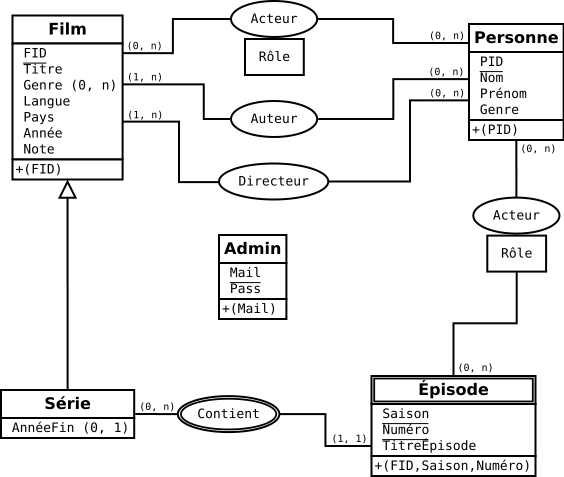
\includegraphics[width=0.8\textwidth]{er.png}
\end{figure}

\subsection{Contraintes d'intégrité}
\begin{list}{-}{}
  \item L'\emph{AnnéeFin} d'une série doit être supérieure à son \emph{Année} (de début).
  \item Une personne ne peut pas jouer deux fois le même rôle dans le même film ou dans le même épisode.
  \item Une personne ne peut pas diriger deux fois le même film.
  \item Une personne ne peut pas écrire deux fois le même film.
\end{list}
\subsection{Remarques}
\begin{list}{-}{}
  \item Il est tout a fait possible qu'un acteur joue plusieurs rôles au sein d'un même film (par exemple dans \emph{Leaves Of Grasses}, Edward Norton y joue le rôle de lui même et de son frère jumeau), ou qu'un rôle soit joué par plusieurs acteurs (comme dans \emph{L'imaginarium du Docteur Parnassus}, où le rôle du personnage principal est interprété par plusieurs acteurs différents au cours du film).
  \item Le type de généralisation pour \emph{Série} n'est pas précisé car c'est la seule sous-entité de \emph{Film}, sa généralisation est donc partielle. Quant à la notion d'exclusivité ou de chevauchement, cela n'a pas de sens dans le cas d'une seule sous-entité.
  \item Une personne ayant joué dans une série aura une entrée dans la relation \emph{Acteur} reliant \emph{Personne} à \emph{Épisode}, et non dans la relation reliant \emph{Personne} à \emph{Film}.
\end{list}

\section{Modèle relationnel}
Film(\underline{FID}, Titre, Pays, Année, Langue, Note)

FilmGenre(\underline{FID, Genre})
\begin{list}{-}{}
  \item FID représente Film.FID
\end{list}

Série(\underline{FID}, AnnéeFin)
\begin{list}{-}{}
  \item FID représente Film.FID
\end{list}

Épisode(\underline{FID, Saison, Numéro}, TitreÉpisode)
\begin{list}{-}{}
  \item FID représente Film.FID
\end{list}

Personne(\underline{PID}, Nom, Prénom, Genre)

ActeurFilm(\underline{FID, PID, Rôle})
\begin{list}{-}{}
  \item FID représente Film.FID
  \item PID représente Personne.PID
\end{list}

Auteur(\underline{FID, PID})
\begin{list}{-}{}
  \item FID représente Film.FID
  \item PID représente Personne.PID
\end{list}

Directeur(\underline{FID, PID})
\begin{list}{-}{}
  \item FID représente Film.FID
  \item PID représente Personne.PID
\end{list}

ActeurSérie(\underline{FID, Saison, Numéro, PID, Rôle})
\begin{list}{-}{}
  \item FID représente Film.FID
  \item Saison représente Série.Saison
  \item Numéro représente Série.Numéro
  \item PID représente Personne.PID
\end{list}

Admin(\underline{Mail}, Pass)
%\section{Remarques}

\end{document}
